\originalchapter{一维谱与变分增补：从完备展开到多点势}
本章补入8.05官方Chapter 1（Barton Zwiebach, Fall 2013）中原册尚未展开的内容. 单点势Gaussian例保留讲义对Griffiths的信用; 中文论证与曲线均为本册独立整理. 先修是一维定态方程、内积和前文已证明的节点定理.
\originalsection{完备关系为何能还原初态}
离散归一能态满足$\int u_n^*u_m\dd x=\delta_{nm}$. 将初态展开后左乘$u_n^*$积分, 得$c_n=\int u_n^*\psi(x,0)\dd x$. 完备性不是只有正交性: 它还要求$\psi=\sum_nc_nu_n$按Hilbert范数收敛. 把系数代回可写核
\[
\sum_nu_n(x)u_n^*(x')=\delta(x-x'),\qquad
\psi(x,t)=\sum_nc_n\e^{-\ii E_nt/\hbar}u_n(x).
\]
第一式按分布或弱意义, 不要求每一点的级数都绝对收敛. 每项相位代回Schrödinger方程给第二式. 归一态$\sum|c_n|^2=1$, 能量测量概率$|c_n|^2$和$\langle H\rangle=\sum E_n|c_n|^2$保持. 有连续谱时还要加$\sum_a\int c_a(E)u_{E,a}\dd E$, $a$为通道, 核与归一式亦添积分项; 只列束缚态不完备.
\originalsection{实势、非简并与奇偶性各有条件}
实势和实能量使$\operatorname{Re}\psi,\operatorname{Im}\psi$各满足同一本征方程. 对普通一维束缚态, Wronskian证明非简并, 故两实部若非零只能成比例, $\psi=\e^{\ii\chi}u$且$u$实. 散射能量可简并, 只保证能选实的本征基, 不保证每个右行波都只是常相位乘实函数.

若势偶, $\Pi\psi(x)=\psi(-x)$保能量. 束缚本征空间一维, $\Pi\psi=c\psi$; $\Pi^2=I$给$c=\pm1$, 所以每个束缚态有确定奇偶. 前文节点数排序使基态偶且无节点, 激发态交替奇偶. 缺少非简并条件时应在简并空间中选择奇偶基, 而不能说任意线性组合都具有确定奇偶.
\originalsection{两端势不同：数清开放通道}
以有限区间外恰为常数的势为例, 设$V_-<V_+$. $E<V_-$时两端均为指数, 正规性只留衰减支; 内部匹配通常只在离散能量可成解. $V_-<E<V_+$时左端是振荡波、右端闭合, 给单个连续入射通道及全反射. $E>V_+$时两端均开放, 可分别从左和右入射, 因而有两个独立连续通道. 左右波数分别$\sqrt{2m(E-V_\pm)}/\hbar$, 计算透射概率须用流比而非只用振幅平方.

在$E=V_\pm$该端解为常数与线性函数, 零能共振或阈值态必须另检查正规性. 以上匹配计数解释有限程示例的谱结构; 对一般渐近势仍需衰减及谱条件, 不能将未知数数量当作无条件谱定理.
\originalsection{五个吸引点势：五峰不等于五节点}
设$V=-g\sum_{j=-2}^2\delta(x-ja)$, $g>0$. 各点导数跳跃$-2mg\psi(ja)/\hbar^2$, 区间负能解是两个实指数的组合, 每段至多一个节点, 两外端衰减支无节点. 至多五个负能态: 如果负能子空间维数至少6, 五个点值条件可在其中选非零组合使所有$\psi(ja)=0$. 其势能为0, 动能非负, 但它又在负能本征态张成空间中有严格负的能量均值, 矛盾.

充分强的$g$时, 在各中心取五个互不交叠的局域试态, 每个点势项随$g$降至负能, 且交叉矩阵元为0. 它们张成的五维子空间Rayleigh商全负, min--max原理给至少五个负本征值, 因而恰五态. 这里min--max的作用可直接理解: 若负本征态少于五个, 在该五维试探子空间可选非零矢正交于所有负态, 谱展开给非负能量均值, 与全负Rayleigh商矛盾. 节点数为0、1、2、3、4, 奇偶依次偶、奇、偶、奇、偶. 本图选$\lambda=mag/\hbar^2=3$作为已声明的数值例, 点间距$a$; 纵向分开画五态, 图不替代全参数证明.
\begin{center}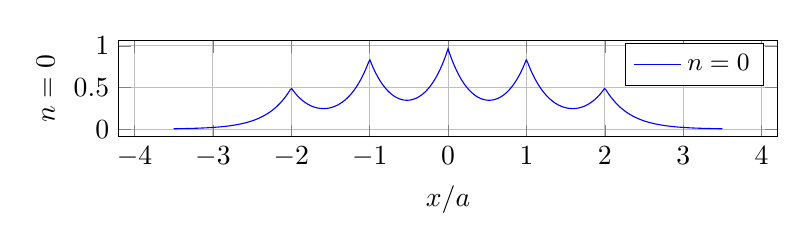
\begin{tikzpicture}
\begin{axis}[width=.82\textwidth,height=2.8cm,xlabel={$x/a$},ylabel={$n=0$},grid=major,legend style={font=\small},]
\addplot+[mark=none] coordinates{(-3.5,0.00397382449) (-3.4825,0.0042037763) (-3.465,0.00444703463) (-3.4475,0.00470436951) (-3.43,0.00497659548) (-3.4125,0.00526457426) (-3.395,0.00556921739) (-3.3775,0.00589148919) (-3.36,0.00623240977) (-3.3425,0.00659305828) (-3.325,0.0069745763) (-3.3075,0.00737817147) (-3.29,0.00780512134) (-3.2725,0.00825677735) (-3.255,0.00873456917) (-3.2375,0.00924000919) (-3.22,0.00977469731) (-3.2025,0.010340326) (-3.185,0.0109386858) (-3.1675,0.0115716706) (-3.15,0.0122412841) (-3.1325,0.0129496458) (-3.115,0.0136989981) (-3.0975,0.0144917129) (-3.08,0.0153302994) (-3.0625,0.016217412) (-3.045,0.0171558589) (-3.0275,0.0181486105) (-3.01,0.0191988093) (-2.9925,0.0203097795) (-2.975,0.0214850379) (-2.9575,0.0227283045) (-2.94,0.0240435147) (-2.9225,0.0254348317) (-2.905,0.0269066595) (-2.8875,0.028463657) (-2.87,0.0301107527) (-2.8525,0.0318531603) (-2.835,0.0336963951) (-2.8175,0.0356462916) (-2.8,0.0377090222) (-2.7825,0.0398911159) (-2.765,0.0421994801) (-2.7475,0.0446414215) (-2.73,0.0472246697) (-2.7125,0.0499574019) (-2.695,0.052848268) (-2.6775,0.0559064188) (-2.66,0.0591415345) (-2.6425,0.0625638553) (-2.625,0.0661842143) (-2.6075,0.0700140713) (-2.59,0.0740655491) (-2.5725,0.0783514723) (-2.555,0.0828854074) (-2.5375,0.087681706) (-2.52,0.0927555502) (-2.5025,0.0981230007) (-2.485,0.103801047) (-2.4675,0.109807663) (-2.45,0.116161862) (-2.4325,0.122883757) (-2.415,0.129994625) (-2.3975,0.137516975) (-2.38,0.145474617) (-2.3625,0.153892742) (-2.345,0.162797995) (-2.3275,0.172218566) (-2.31,0.182184272) (-2.2925,0.192726661) (-2.275,0.203879102) (-2.2575,0.215676897) (-2.24,0.228157391) (-2.2225,0.241360088) (-2.205,0.255326781) (-2.1875,0.27010168) (-2.17,0.285731552) (-2.1525,0.302265872) (-2.135,0.319756977) (-2.1175,0.338260233) (-2.1,0.357834211) (-2.0825,0.378540868) (-2.065,0.40044575) (-2.0475,0.423618193) (-2.03,0.448131547) (-2.0125,0.474063406) (-1.995,0.486690219) (-1.9775,0.463835136) (-1.96,0.442448265) (-1.9425,0.422461909) (-1.925,0.403812805) (-1.9075,0.38644192) (-1.89,0.370294269) (-1.8725,0.355318739) (-1.855,0.341467926) (-1.8375,0.328697988) (-1.82,0.316968503) (-1.8025,0.306242342) (-1.785,0.296485554) (-1.7675,0.287667254) (-1.75,0.279759529) (-1.7325,0.272737348) (-1.715,0.266578484) (-1.6975,0.261263441) (-1.68,0.256775395) (-1.6625,0.253100139) (-1.645,0.250226041) (-1.6275,0.248144003) (-1.61,0.246847434) (-1.5925,0.24633223) (-1.575,0.24659676) (-1.5575,0.247641861) (-1.54,0.249470843) (-1.5225,0.252089493) (-1.505,0.255506102) (-1.4875,0.259731483) (-1.47,0.264779013) (-1.4525,0.270664667) (-1.435,0.277407077) (-1.4175,0.285027585) (-1.4,0.293550313) (-1.3825,0.303002238) (-1.365,0.313413279) (-1.3475,0.324816391) (-1.33,0.337247669) (-1.3125,0.350746463) (-1.295,0.365355501) (-1.2775,0.381121027) (-1.26,0.398092945) (-1.2425,0.416324977) (-1.225,0.435874834) (-1.2075,0.456804398) (-1.19,0.479179921) (-1.1725,0.503072229) (-1.155,0.528556949) (-1.1375,0.555714751) (-1.12,0.5846316) (-1.1025,0.615399027) (-1.085,0.648114424) (-1.0675,0.682881347) (-1.05,0.719809847) (-1.0325,0.759016816) (-1.015,0.800626358) (-0.9975,0.832195496) (-0.98,0.790922287) (-0.9625,0.752152644) (-0.945,0.715763848) (-0.9275,0.681640713) (-0.91,0.649675228) (-0.8925,0.61976621) (-0.875,0.591818985) (-0.8575,0.56574509) (-0.84,0.541461991) (-0.8225,0.518892823) (-0.805,0.497966146) (-0.7875,0.478615719) (-0.77,0.460780291) (-0.7525,0.444403407) (-0.735,0.429433226) (-0.7175,0.415822363) (-0.7,0.403527734) (-0.6825,0.392510423) (-0.665,0.382735555) (-0.6475,0.374172189) (-0.63,0.366793218) (-0.6125,0.360575287) (-0.595,0.355498711) (-0.5775,0.351547423) (-0.56,0.348708915) (-0.5425,0.346974202) (-0.525,0.346337793) (-0.5075,0.346797673) (-0.49,0.348355299) (-0.4725,0.3510156) (-0.455,0.354786997) (-0.4375,0.359681429) (-0.42,0.365714388) (-0.4025,0.372904971) (-0.385,0.381275938) (-0.3675,0.390853788) (-0.35,0.401668836) (-0.3325,0.413755318) (-0.315,0.427151491) (-0.2975,0.441899759) (-0.28,0.458046806) (-0.2625,0.475643744) (-0.245,0.494746273) (-0.2275,0.51541486) (-0.21,0.53771493) (-0.1925,0.561717069) (-0.175,0.587497255) (-0.1575,0.61513709) (-0.14,0.644724066) (-0.1225,0.676351836) (-0.105,0.710120515) (-0.0875,0.746136992) (-0.07,0.784515273) (-0.0525,0.825376841) (-0.035,0.868851037) (-0.0175,0.915075473) (4.4408921e-16,0.964196468) (0.0175,0.915075473) (0.035,0.868851037) (0.0525,0.825376841) (0.07,0.784515273) (0.0875,0.746136992) (0.105,0.710120515) (0.1225,0.676351836) (0.14,0.644724066) (0.1575,0.61513709) (0.175,0.587497255) (0.1925,0.561717069) (0.21,0.53771493) (0.2275,0.51541486) (0.245,0.494746273) (0.2625,0.475643744) (0.28,0.458046806) (0.2975,0.441899759) (0.315,0.427151491) (0.3325,0.413755318) (0.35,0.401668836) (0.3675,0.390853788) (0.385,0.381275938) (0.4025,0.372904971) (0.42,0.365714388) (0.4375,0.359681429) (0.455,0.354786997) (0.4725,0.3510156) (0.49,0.348355299) (0.5075,0.346797673) (0.525,0.346337793) (0.5425,0.346974202) (0.56,0.348708915) (0.5775,0.351547423) (0.595,0.355498711) (0.6125,0.360575287) (0.63,0.366793218) (0.6475,0.374172189) (0.665,0.382735555) (0.6825,0.392510423) (0.7,0.403527734) (0.7175,0.415822363) (0.735,0.429433226) (0.7525,0.444403407) (0.77,0.460780291) (0.7875,0.478615719) (0.805,0.497966146) (0.8225,0.518892823) (0.84,0.541461991) (0.8575,0.56574509) (0.875,0.591818985) (0.8925,0.61976621) (0.91,0.649675228) (0.9275,0.681640713) (0.945,0.715763848) (0.9625,0.752152644) (0.98,0.790922287) (0.9975,0.832195496) (1.015,0.800626358) (1.0325,0.759016816) (1.05,0.719809847) (1.0675,0.682881347) (1.085,0.648114424) (1.1025,0.615399027) (1.12,0.5846316) (1.1375,0.555714751) (1.155,0.528556949) (1.1725,0.503072229) (1.19,0.479179921) (1.2075,0.456804398) (1.225,0.435874834) (1.2425,0.416324977) (1.26,0.398092945) (1.2775,0.381121027) (1.295,0.365355501) (1.3125,0.350746463) (1.33,0.337247669) (1.3475,0.324816391) (1.365,0.313413279) (1.3825,0.303002238) (1.4,0.293550313) (1.4175,0.285027585) (1.435,0.277407077) (1.4525,0.270664667) (1.47,0.264779013) (1.4875,0.259731483) (1.505,0.255506102) (1.5225,0.252089493) (1.54,0.249470843) (1.5575,0.247641861) (1.575,0.24659676) (1.5925,0.24633223) (1.61,0.246847434) (1.6275,0.248144003) (1.645,0.250226041) (1.6625,0.253100139) (1.68,0.256775395) (1.6975,0.261263441) (1.715,0.266578484) (1.7325,0.272737348) (1.75,0.279759529) (1.7675,0.287667254) (1.785,0.296485554) (1.8025,0.306242342) (1.82,0.316968503) (1.8375,0.328697988) (1.855,0.341467926) (1.8725,0.355318739) (1.89,0.370294269) (1.9075,0.38644192) (1.925,0.403812805) (1.9425,0.422461909) (1.96,0.442448265) (1.9775,0.463835136) (1.995,0.486690219) (2.0125,0.474063406) (2.03,0.448131547) (2.0475,0.423618193) (2.065,0.40044575) (2.0825,0.378540868) (2.1,0.357834211) (2.1175,0.338260233) (2.135,0.319756977) (2.1525,0.302265872) (2.17,0.285731552) (2.1875,0.27010168) (2.205,0.255326781) (2.2225,0.241360088) (2.24,0.228157391) (2.2575,0.215676897) (2.275,0.203879102) (2.2925,0.192726661) (2.31,0.182184272) (2.3275,0.172218566) (2.345,0.162797995) (2.3625,0.153892742) (2.38,0.145474617) (2.3975,0.137516975) (2.415,0.129994625) (2.4325,0.122883757) (2.45,0.116161862) (2.4675,0.109807663) (2.485,0.103801047) (2.5025,0.0981230007) (2.52,0.0927555502) (2.5375,0.087681706) (2.555,0.0828854074) (2.5725,0.0783514723) (2.59,0.0740655491) (2.6075,0.0700140713) (2.625,0.0661842143) (2.6425,0.0625638553) (2.66,0.0591415345) (2.6775,0.0559064188) (2.695,0.052848268) (2.7125,0.0499574019) (2.73,0.0472246697) (2.7475,0.0446414215) (2.765,0.0421994801) (2.7825,0.0398911159) (2.8,0.0377090222) (2.8175,0.0356462916) (2.835,0.0336963951) (2.8525,0.0318531603) (2.87,0.0301107527) (2.8875,0.028463657) (2.905,0.0269066595) (2.9225,0.0254348317) (2.94,0.0240435147) (2.9575,0.0227283045) (2.975,0.0214850379) (2.9925,0.0203097795) (3.01,0.0191988093) (3.0275,0.0181486105) (3.045,0.0171558589) (3.0625,0.016217412) (3.08,0.0153302994) (3.0975,0.0144917129) (3.115,0.0136989981) (3.1325,0.0129496458) (3.15,0.0122412841) (3.1675,0.0115716706) (3.185,0.0109386858) (3.2025,0.010340326) (3.22,0.00977469731) (3.2375,0.00924000919) (3.255,0.00873456917) (3.2725,0.00825677735) (3.29,0.00780512134) (3.3075,0.00737817147) (3.325,0.0069745763) (3.3425,0.00659305828) (3.36,0.00623240977) (3.3775,0.00589148919) (3.395,0.00556921739) (3.4125,0.00526457426) (3.43,0.00497659548) (3.4475,0.00470436951) (3.465,0.00444703463) (3.4825,0.0042037763) (3.5,0.00397382449)};
\addlegendentry{$n=0$}
\end{axis}\end{tikzpicture}\end{center}
\begin{center}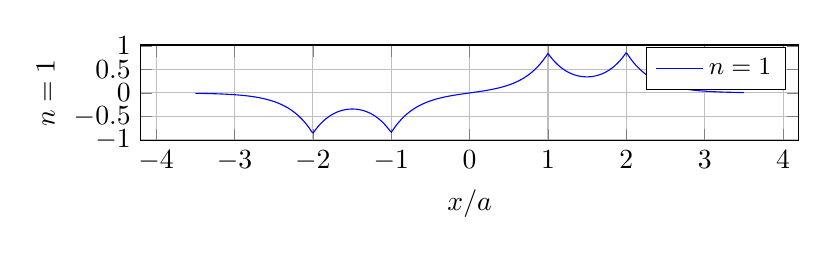
\begin{tikzpicture}
\begin{axis}[width=.82\textwidth,height=2.8cm,xlabel={$x/a$},ylabel={$n=1$},grid=major,legend style={font=\small},]
\addplot+[mark=none] coordinates{(-3.5,-0.00788790698) (-3.4825,-0.00833176792) (-3.465,-0.00880060538) (-3.4475,-0.00929582482) (-3.43,-0.0098189108) (-3.4125,-0.0103714314) (-3.395,-0.0109550429) (-3.3775,-0.0115714948) (-3.36,-0.0122226352) (-3.3425,-0.0129104159) (-3.325,-0.0136368987) (-3.3075,-0.0144042616) (-3.29,-0.0152148047) (-3.2725,-0.016070958) (-3.255,-0.0169752879) (-3.2375,-0.0179305055) (-3.22,-0.0189394741) (-3.2025,-0.0200052185) (-3.185,-0.0211309335) (-3.1675,-0.0223199937) (-3.15,-0.0235759635) (-3.1325,-0.0249026081) (-3.115,-0.0263039044) (-3.0975,-0.0277840531) (-3.08,-0.0293474914) (-3.0625,-0.030998906) (-3.045,-0.0327432475) (-3.0275,-0.034585745) (-3.01,-0.0365319217) (-2.9925,-0.0385876119) (-2.975,-0.0407589779) (-2.9575,-0.043052529) (-2.94,-0.0454751408) (-2.9225,-0.0480340754) (-2.905,-0.050737004) (-2.8875,-0.0535920293) (-2.87,-0.0566077099) (-2.8525,-0.0597930861) (-2.835,-0.0631577068) (-2.8175,-0.0667116583) (-2.8,-0.0704655944) (-2.7825,-0.0744307685) (-2.765,-0.0786190672) (-2.7475,-0.0830430459) (-2.73,-0.0877159666) (-2.7125,-0.0926518376) (-2.695,-0.0978654552) (-2.6775,-0.103372449) (-2.66,-0.109189327) (-2.6425,-0.115333526) (-2.625,-0.121823467) (-2.6075,-0.128678603) (-2.59,-0.135919485) (-2.5725,-0.14356782) (-2.555,-0.151646534) (-2.5375,-0.160179846) (-2.52,-0.169193337) (-2.5025,-0.178714026) (-2.485,-0.188770455) (-2.4675,-0.19939277) (-2.45,-0.210612813) (-2.4325,-0.222464221) (-2.415,-0.23498252) (-2.3975,-0.248205236) (-2.38,-0.26217201) (-2.3625,-0.276924708) (-2.345,-0.292507557) (-2.3275,-0.308967269) (-2.31,-0.326353186) (-2.2925,-0.344717428) (-2.275,-0.364115045) (-2.2575,-0.384604187) (-2.24,-0.406246274) (-2.2225,-0.429106185) (-2.205,-0.453252448) (-2.1875,-0.478757446) (-2.17,-0.505697638) (-2.1525,-0.534153783) (-2.135,-0.564211186) (-2.1175,-0.59595995) (-2.1,-0.629495252) (-2.0825,-0.664917621) (-2.065,-0.702333244) (-2.0475,-0.741854285) (-2.03,-0.783599216) (-2.0125,-0.827693179) (-1.995,-0.848446304) (-1.9775,-0.807173906) (-1.96,-0.76832121) (-1.9425,-0.731771746) (-1.925,-0.697415948) (-1.9075,-0.665150827) (-1.89,-0.634879659) (-1.8725,-0.606511699) (-1.855,-0.579961908) (-1.8375,-0.555150696) (-1.82,-0.532003684) (-1.8025,-0.510451485) (-1.785,-0.49042949) (-1.7675,-0.471877678) (-1.75,-0.454740436) (-1.7325,-0.43896639) (-1.715,-0.424508254) (-1.6975,-0.411322686) (-1.68,-0.39937016) (-1.6625,-0.388614844) (-1.645,-0.379024497) (-1.6275,-0.370570369) (-1.61,-0.363227117) (-1.5925,-0.356972728) (-1.575,-0.351788452) (-1.5575,-0.34765875) (-1.54,-0.34457124) (-1.5225,-0.342516667) (-1.505,-0.341488872) (-1.4875,-0.341484775) (-1.47,-0.342504362) (-1.4525,-0.34455069) (-1.435,-0.347629895) (-1.4175,-0.351751205) (-1.4,-0.356926976) (-1.3825,-0.363172724) (-1.365,-0.370507172) (-1.3475,-0.378952306) (-1.33,-0.388533443) (-1.3125,-0.399279305) (-1.295,-0.411222105) (-1.2775,-0.424397645) (-1.26,-0.438845421) (-1.2425,-0.454608745) (-1.225,-0.47173487) (-1.2075,-0.490275137) (-1.19,-0.510285124) (-1.1725,-0.531824817) (-1.155,-0.554958786) (-1.1375,-0.57975638) (-1.12,-0.606291937) (-1.1025,-0.634645004) (-1.085,-0.664900575) (-1.0675,-0.69714935) (-1.05,-0.731488002) (-1.0325,-0.76801947) (-1.015,-0.806853265) (-0.9975,-0.835474774) (-0.98,-0.790787621) (-0.9625,-0.748471048) (-0.945,-0.708398201) (-0.9275,-0.670448953) (-0.91,-0.634509541) (-0.8925,-0.600472227) (-0.875,-0.568234977) (-0.8575,-0.537701152) (-0.84,-0.508779218) (-0.8225,-0.481382475) (-0.805,-0.455428795) (-0.7875,-0.430840375) (-0.77,-0.407543505) (-0.7525,-0.385468347) (-0.735,-0.364548726) (-0.7175,-0.344721929) (-0.7,-0.325928521) (-0.6825,-0.308112164) (-0.665,-0.29121945) (-0.6475,-0.275199737) (-0.63,-0.260005004) (-0.6125,-0.245589699) (-0.595,-0.231910611) (-0.5775,-0.218926731) (-0.56,-0.206599138) (-0.5425,-0.194890878) (-0.525,-0.18376685) (-0.5075,-0.173193709) (-0.49,-0.163139759) (-0.4725,-0.153574861) (-0.455,-0.144470341) (-0.4375,-0.135798906) (-0.42,-0.127534562) (-0.4025,-0.119652535) (-0.385,-0.112129195) (-0.3675,-0.10494199) (-0.35,-0.098069375) (-0.3325,-0.0914907469) (-0.315,-0.0851863848) (-0.2975,-0.07913739) (-0.28,-0.0733256289) (-0.2625,-0.0677336795) (-0.245,-0.0623447786) (-0.2275,-0.0571427714) (-0.21,-0.0521120638) (-0.1925,-0.047237575) (-0.175,-0.0425046924) (-0.1575,-0.0378992281) (-0.14,-0.0334073761) (-0.1225,-0.0290156709) (-0.105,-0.0247109474) (-0.0875,-0.020480301) (-0.07,-0.0163110494) (-0.0525,-0.0121906941) (-0.035,-0.0081068835) (-0.0175,-0.00404737525) (4.4408921e-16,1.63442063e-16) (0.0175,0.00404737525) (0.035,0.0081068835) (0.0525,0.0121906941) (0.07,0.0163110494) (0.0875,0.020480301) (0.105,0.0247109474) (0.1225,0.0290156709) (0.14,0.0334073761) (0.1575,0.0378992281) (0.175,0.0425046924) (0.1925,0.047237575) (0.21,0.0521120638) (0.2275,0.0571427714) (0.245,0.0623447786) (0.2625,0.0677336795) (0.28,0.0733256289) (0.2975,0.07913739) (0.315,0.0851863848) (0.3325,0.0914907469) (0.35,0.098069375) (0.3675,0.10494199) (0.385,0.112129195) (0.4025,0.119652535) (0.42,0.127534562) (0.4375,0.135798906) (0.455,0.144470341) (0.4725,0.153574861) (0.49,0.163139759) (0.5075,0.173193709) (0.525,0.18376685) (0.5425,0.194890878) (0.56,0.206599138) (0.5775,0.218926731) (0.595,0.231910611) (0.6125,0.245589699) (0.63,0.260005004) (0.6475,0.275199737) (0.665,0.29121945) (0.6825,0.308112164) (0.7,0.325928521) (0.7175,0.344721929) (0.735,0.364548726) (0.7525,0.385468347) (0.77,0.407543505) (0.7875,0.430840375) (0.805,0.455428795) (0.8225,0.481382475) (0.84,0.508779218) (0.8575,0.537701152) (0.875,0.568234977) (0.8925,0.600472227) (0.91,0.634509541) (0.9275,0.670448953) (0.945,0.708398201) (0.9625,0.748471048) (0.98,0.790787621) (0.9975,0.835474774) (1.015,0.806853265) (1.0325,0.76801947) (1.05,0.731488002) (1.0675,0.69714935) (1.085,0.664900575) (1.1025,0.634645004) (1.12,0.606291937) (1.1375,0.57975638) (1.155,0.554958786) (1.1725,0.531824817) (1.19,0.510285124) (1.2075,0.490275137) (1.225,0.47173487) (1.2425,0.454608745) (1.26,0.438845421) (1.2775,0.424397645) (1.295,0.411222105) (1.3125,0.399279305) (1.33,0.388533443) (1.3475,0.378952306) (1.365,0.370507172) (1.3825,0.363172724) (1.4,0.356926976) (1.4175,0.351751205) (1.435,0.347629895) (1.4525,0.34455069) (1.47,0.342504362) (1.4875,0.341484775) (1.505,0.341488872) (1.5225,0.342516667) (1.54,0.34457124) (1.5575,0.34765875) (1.575,0.351788452) (1.5925,0.356972728) (1.61,0.363227117) (1.6275,0.370570369) (1.645,0.379024497) (1.6625,0.388614844) (1.68,0.39937016) (1.6975,0.411322686) (1.715,0.424508254) (1.7325,0.43896639) (1.75,0.454740436) (1.7675,0.471877678) (1.785,0.49042949) (1.8025,0.510451485) (1.82,0.532003684) (1.8375,0.555150696) (1.855,0.579961908) (1.8725,0.606511699) (1.89,0.634879659) (1.9075,0.665150827) (1.925,0.697415948) (1.9425,0.731771746) (1.96,0.76832121) (1.9775,0.807173906) (1.995,0.848446304) (2.0125,0.827693179) (2.03,0.783599216) (2.0475,0.741854285) (2.065,0.702333244) (2.0825,0.664917621) (2.1,0.629495252) (2.1175,0.59595995) (2.135,0.564211186) (2.1525,0.534153783) (2.17,0.505697638) (2.1875,0.478757446) (2.205,0.453252448) (2.2225,0.429106185) (2.24,0.406246274) (2.2575,0.384604187) (2.275,0.364115045) (2.2925,0.344717428) (2.31,0.326353186) (2.3275,0.308967269) (2.345,0.292507557) (2.3625,0.276924708) (2.38,0.26217201) (2.3975,0.248205236) (2.415,0.23498252) (2.4325,0.222464221) (2.45,0.210612813) (2.4675,0.19939277) (2.485,0.188770455) (2.5025,0.178714026) (2.52,0.169193337) (2.5375,0.160179846) (2.555,0.151646534) (2.5725,0.14356782) (2.59,0.135919485) (2.6075,0.128678603) (2.625,0.121823467) (2.6425,0.115333526) (2.66,0.109189327) (2.6775,0.103372449) (2.695,0.0978654552) (2.7125,0.0926518376) (2.73,0.0877159666) (2.7475,0.0830430459) (2.765,0.0786190672) (2.7825,0.0744307685) (2.8,0.0704655944) (2.8175,0.0667116583) (2.835,0.0631577068) (2.8525,0.0597930861) (2.87,0.0566077099) (2.8875,0.0535920293) (2.905,0.050737004) (2.9225,0.0480340754) (2.94,0.0454751408) (2.9575,0.043052529) (2.975,0.0407589779) (2.9925,0.0385876119) (3.01,0.0365319217) (3.0275,0.034585745) (3.045,0.0327432475) (3.0625,0.030998906) (3.08,0.0293474914) (3.0975,0.0277840531) (3.115,0.0263039044) (3.1325,0.0249026081) (3.15,0.0235759635) (3.1675,0.0223199937) (3.185,0.0211309335) (3.2025,0.0200052185) (3.22,0.0189394741) (3.2375,0.0179305055) (3.255,0.0169752879) (3.2725,0.016070958) (3.29,0.0152148047) (3.3075,0.0144042616) (3.325,0.0136368987) (3.3425,0.0129104159) (3.36,0.0122226352) (3.3775,0.0115714948) (3.395,0.0109550429) (3.4125,0.0103714314) (3.43,0.0098189108) (3.4475,0.00929582482) (3.465,0.00880060538) (3.4825,0.00833176792) (3.5,0.00788790698)};
\addlegendentry{$n=1$}
\end{axis}\end{tikzpicture}\end{center}
\begin{center}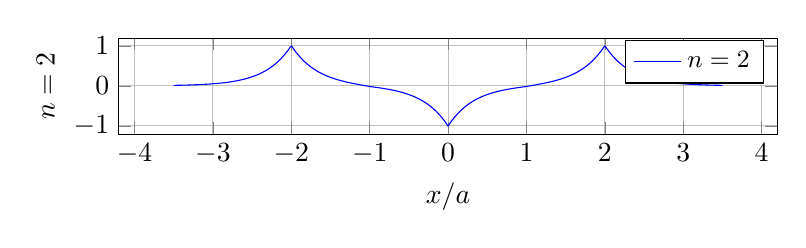
\begin{tikzpicture}
\begin{axis}[width=.82\textwidth,height=2.8cm,xlabel={$x/a$},ylabel={$n=2$},grid=major,legend style={font=\small},]
\addplot+[mark=none] coordinates{(-3.5,0.0113528548) (-3.4825,0.0119626861) (-3.465,0.0126052751) (-3.4475,0.0132823816) (-3.43,0.0139958596) (-3.4125,0.0147476628) (-3.395,0.01553985) (-3.3775,0.0163745904) (-3.36,0.0172541698) (-3.3425,0.0181809968) (-3.325,0.0191576094) (-3.3075,0.0201866818) (-3.29,0.021271032) (-3.2725,0.0224136293) (-3.255,0.0236176024) (-3.2375,0.0248862483) (-3.22,0.026223041) (-3.2025,0.0276316409) (-3.185,0.0291159054) (-3.1675,0.0306798988) (-3.15,0.0323279039) (-3.1325,0.0340644334) (-3.115,0.0358942425) (-3.0975,0.0378223418) (-3.08,0.0398540112) (-3.0625,0.041994814) (-3.045,0.0442506123) (-3.0275,0.0466275834) (-3.01,0.0491322362) (-2.9925,0.0517714292) (-2.975,0.0545523894) (-2.9575,0.0574827319) (-2.94,0.0605704811) (-2.9225,0.0638240922) (-2.905,0.0672524747) (-2.8875,0.0708650165) (-2.87,0.0746716101) (-2.8525,0.0786826791) (-2.835,0.0829092072) (-2.8175,0.0873627679) (-2.8,0.0920555566) (-2.7825,0.0970004238) (-2.765,0.10221091) (-2.7475,0.107701283) (-2.73,0.113486578) (-2.7125,0.119582636) (-2.695,0.126006151) (-2.6775,0.132774713) (-2.66,0.139906855) (-2.6425,0.147422108) (-2.625,0.155341051) (-2.6075,0.163685369) (-2.59,0.172477912) (-2.5725,0.181742756) (-2.555,0.191505271) (-2.5375,0.201792191) (-2.52,0.212631684) (-2.5025,0.224053432) (-2.485,0.236088713) (-2.4675,0.248770482) (-2.45,0.262133467) (-2.4325,0.276214259) (-2.415,0.291051416) (-2.3975,0.306685569) (-2.38,0.323159527) (-2.3625,0.340518402) (-2.345,0.358809729) (-2.3275,0.378083594) (-2.31,0.398392777) (-2.2925,0.41979289) (-2.275,0.442342535) (-2.2575,0.466103458) (-2.24,0.491140727) (-2.2225,0.5175229) (-2.205,0.545322221) (-2.1875,0.574614813) (-2.17,0.60548089) (-2.1525,0.638004973) (-2.135,0.672276124) (-2.1175,0.708388187) (-2.1,0.74644005) (-2.0825,0.786535912) (-2.065,0.828785568) (-2.0475,0.873304711) (-2.03,0.920215249) (-2.0125,0.96964564) (-1.995,0.991532999) (-1.9775,0.940625136) (-1.96,0.892293015) (-1.9425,0.846404285) (-1.925,0.802833288) (-1.9075,0.761460713) (-1.89,0.722173268) (-1.8725,0.684863371) (-1.855,0.649428855) (-1.8375,0.615772689) (-1.82,0.583802711) (-1.8025,0.553431376) (-1.785,0.524575519) (-1.7675,0.497156123) (-1.75,0.471098103) (-1.7325,0.446330105) (-1.715,0.422784305) (-1.6975,0.400396228) (-1.68,0.379104567) (-1.6625,0.35885102) (-1.645,0.339580124) (-1.6275,0.321239111) (-1.61,0.303777756) (-1.5925,0.287148244) (-1.575,0.271305039) (-1.5575,0.256204756) (-1.54,0.241806046) (-1.5225,0.228069481) (-1.505,0.214957445) (-1.4875,0.202434033) (-1.47,0.190464952) (-1.4525,0.179017426) (-1.435,0.16806011) (-1.4175,0.157562997) (-1.4,0.147497343) (-1.3825,0.137835586) (-1.365,0.128551268) (-1.3475,0.119618965) (-1.33,0.111014219) (-1.3125,0.102713466) (-1.295,0.0946939759) (-1.2775,0.0869337894) (-1.26,0.0794116562) (-1.2425,0.0721069782) (-1.225,0.0649997529) (-1.2075,0.0580705182) (-1.19,0.0513002998) (-1.1725,0.0446705584) (-1.155,0.0381631397) (-1.1375,0.0317602243) (-1.12,0.0254442788) (-1.1025,0.019198008) (-1.085,0.0130043078) (-1.0675,0.00684621761) (-1.05,0.000706874625) (-1.0325,-0.0054305327) (-1.015,-0.0115828106) (-0.9975,-0.0175135918) (-0.98,-0.02197255) (-0.9625,-0.0264916762) (-0.945,-0.0310833454) (-0.9275,-0.035760131) (-0.91,-0.0405348395) (-0.8925,-0.0454205459) (-0.875,-0.0504306286) (-0.8575,-0.0555788069) (-0.84,-0.0608791783) (-0.8225,-0.066346257) (-0.805,-0.0719950134) (-0.7875,-0.077840916) (-0.77,-0.0838999725) (-0.7525,-0.0901887748) (-0.735,-0.0967245436) (-0.7175,-0.103525176) (-0.7,-0.110609294) (-0.6825,-0.117996297) (-0.665,-0.125706413) (-0.6475,-0.133760754) (-0.63,-0.142181377) (-0.6125,-0.150991338) (-0.595,-0.160214763) (-0.5775,-0.16987691) (-0.56,-0.180004235) (-0.5425,-0.190624471) (-0.525,-0.201766699) (-0.5075,-0.213461431) (-0.49,-0.22574069) (-0.4725,-0.238638102) (-0.455,-0.252188984) (-0.4375,-0.266430441) (-0.42,-0.281401473) (-0.4025,-0.297143075) (-0.385,-0.313698352) (-0.3675,-0.331112639) (-0.35,-0.349433621) (-0.3325,-0.368711467) (-0.315,-0.388998966) (-0.2975,-0.410351672) (-0.28,-0.432828056) (-0.2625,-0.456489666) (-0.245,-0.481401295) (-0.2275,-0.507631159) (-0.21,-0.535251083) (-0.1925,-0.564336702) (-0.175,-0.59496766) (-0.1575,-0.627227835) (-0.14,-0.661205566) (-0.1225,-0.696993895) (-0.105,-0.734690823) (-0.0875,-0.774399576) (-0.07,-0.81622889) (-0.0525,-0.860293307) (-0.035,-0.90671349) (-0.0175,-0.955616553) (4.4408921e-16,-1.00713641) (0.0175,-0.955616553) (0.035,-0.90671349) (0.0525,-0.860293307) (0.07,-0.81622889) (0.0875,-0.774399576) (0.105,-0.734690823) (0.1225,-0.696993895) (0.14,-0.661205566) (0.1575,-0.627227835) (0.175,-0.59496766) (0.1925,-0.564336702) (0.21,-0.535251083) (0.2275,-0.507631159) (0.245,-0.481401295) (0.2625,-0.456489666) (0.28,-0.432828056) (0.2975,-0.410351672) (0.315,-0.388998966) (0.3325,-0.368711467) (0.35,-0.349433621) (0.3675,-0.331112639) (0.385,-0.313698352) (0.4025,-0.297143075) (0.42,-0.281401473) (0.4375,-0.266430441) (0.455,-0.252188984) (0.4725,-0.238638102) (0.49,-0.22574069) (0.5075,-0.213461431) (0.525,-0.201766699) (0.5425,-0.190624471) (0.56,-0.180004235) (0.5775,-0.16987691) (0.595,-0.160214763) (0.6125,-0.150991338) (0.63,-0.142181377) (0.6475,-0.133760754) (0.665,-0.125706413) (0.6825,-0.117996297) (0.7,-0.110609294) (0.7175,-0.103525176) (0.735,-0.0967245436) (0.7525,-0.0901887748) (0.77,-0.0838999725) (0.7875,-0.077840916) (0.805,-0.0719950134) (0.8225,-0.066346257) (0.84,-0.0608791783) (0.8575,-0.0555788069) (0.875,-0.0504306286) (0.8925,-0.0454205459) (0.91,-0.0405348395) (0.9275,-0.035760131) (0.945,-0.0310833454) (0.9625,-0.0264916762) (0.98,-0.02197255) (0.9975,-0.0175135918) (1.015,-0.0115828106) (1.0325,-0.0054305327) (1.05,0.000706874625) (1.0675,0.00684621761) (1.085,0.0130043078) (1.1025,0.019198008) (1.12,0.0254442788) (1.1375,0.0317602243) (1.155,0.0381631397) (1.1725,0.0446705584) (1.19,0.0513002998) (1.2075,0.0580705182) (1.225,0.0649997529) (1.2425,0.0721069782) (1.26,0.0794116562) (1.2775,0.0869337894) (1.295,0.0946939759) (1.3125,0.102713466) (1.33,0.111014219) (1.3475,0.119618965) (1.365,0.128551268) (1.3825,0.137835586) (1.4,0.147497343) (1.4175,0.157562997) (1.435,0.16806011) (1.4525,0.179017426) (1.47,0.190464952) (1.4875,0.202434033) (1.505,0.214957445) (1.5225,0.228069481) (1.54,0.241806046) (1.5575,0.256204756) (1.575,0.271305039) (1.5925,0.287148244) (1.61,0.303777756) (1.6275,0.321239111) (1.645,0.339580124) (1.6625,0.35885102) (1.68,0.379104567) (1.6975,0.400396228) (1.715,0.422784305) (1.7325,0.446330105) (1.75,0.471098103) (1.7675,0.497156123) (1.785,0.524575519) (1.8025,0.553431376) (1.82,0.583802711) (1.8375,0.615772689) (1.855,0.649428855) (1.8725,0.684863371) (1.89,0.722173268) (1.9075,0.761460713) (1.925,0.802833288) (1.9425,0.846404285) (1.96,0.892293015) (1.9775,0.940625136) (1.995,0.991532999) (2.0125,0.96964564) (2.03,0.920215249) (2.0475,0.873304711) (2.065,0.828785568) (2.0825,0.786535912) (2.1,0.74644005) (2.1175,0.708388187) (2.135,0.672276124) (2.1525,0.638004973) (2.17,0.60548089) (2.1875,0.574614813) (2.205,0.545322221) (2.2225,0.5175229) (2.24,0.491140727) (2.2575,0.466103458) (2.275,0.442342535) (2.2925,0.41979289) (2.31,0.398392777) (2.3275,0.378083594) (2.345,0.358809729) (2.3625,0.340518402) (2.38,0.323159527) (2.3975,0.306685569) (2.415,0.291051416) (2.4325,0.276214259) (2.45,0.262133467) (2.4675,0.248770482) (2.485,0.236088713) (2.5025,0.224053432) (2.52,0.212631684) (2.5375,0.201792191) (2.555,0.191505271) (2.5725,0.181742756) (2.59,0.172477912) (2.6075,0.163685369) (2.625,0.155341051) (2.6425,0.147422108) (2.66,0.139906855) (2.6775,0.132774713) (2.695,0.126006151) (2.7125,0.119582636) (2.73,0.113486578) (2.7475,0.107701283) (2.765,0.10221091) (2.7825,0.0970004238) (2.8,0.0920555566) (2.8175,0.0873627679) (2.835,0.0829092072) (2.8525,0.0786826791) (2.87,0.0746716101) (2.8875,0.0708650165) (2.905,0.0672524747) (2.9225,0.0638240922) (2.94,0.0605704811) (2.9575,0.0574827319) (2.975,0.0545523894) (2.9925,0.0517714292) (3.01,0.0491322362) (3.0275,0.0466275834) (3.045,0.0442506123) (3.0625,0.041994814) (3.08,0.0398540112) (3.0975,0.0378223418) (3.115,0.0358942425) (3.1325,0.0340644334) (3.15,0.0323279039) (3.1675,0.0306798988) (3.185,0.0291159054) (3.2025,0.0276316409) (3.22,0.026223041) (3.2375,0.0248862483) (3.255,0.0236176024) (3.2725,0.0224136293) (3.29,0.021271032) (3.3075,0.0201866818) (3.325,0.0191576094) (3.3425,0.0181809968) (3.36,0.0172541698) (3.3775,0.0163745904) (3.395,0.01553985) (3.4125,0.0147476628) (3.43,0.0139958596) (3.4475,0.0132823816) (3.465,0.0126052751) (3.4825,0.0119626861) (3.5,0.0113528548)};
\addlegendentry{$n=2$}
\end{axis}\end{tikzpicture}\end{center}
\begin{center}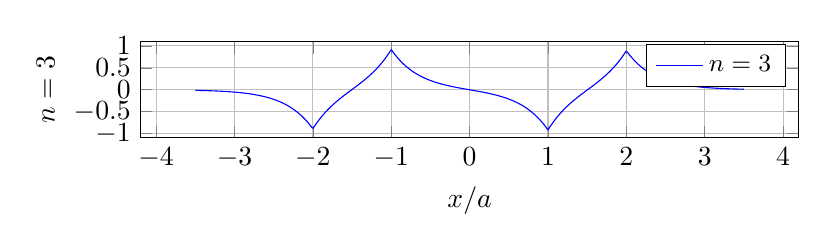
\begin{tikzpicture}
\begin{axis}[width=.82\textwidth,height=2.8cm,xlabel={$x/a$},ylabel={$n=3$},grid=major,legend style={font=\small},]
\addplot+[mark=none] coordinates{(-3.5,-0.0130206174) (-3.4825,-0.0136782396) (-3.465,-0.0143690759) (-3.4475,-0.0150948038) (-3.43,-0.0158571854) (-3.4125,-0.016658072) (-3.395,-0.0174994084) (-3.3775,-0.0183832375) (-3.36,-0.0193117055) (-3.3425,-0.020287067) (-3.325,-0.0213116902) (-3.3075,-0.0223880633) (-3.29,-0.0235188) (-3.2725,-0.0247066459) (-3.255,-0.0259544854) (-3.2375,-0.0272653485) (-3.22,-0.0286424185) (-3.2025,-0.030089039) (-3.185,-0.0316087229) (-3.1675,-0.0332051603) (-3.15,-0.0348822277) (-3.1325,-0.0366439975) (-3.115,-0.0384947476) (-3.0975,-0.0404389722) (-3.08,-0.0424813922) (-3.0625,-0.0446269671) (-3.045,-0.0468809069) (-3.0275,-0.0492486847) (-3.01,-0.05173605) (-2.9925,-0.0543490428) (-2.975,-0.057094008) (-2.9575,-0.0599776111) (-2.94,-0.063006854) (-2.9225,-0.0661890926) (-2.905,-0.069532054) (-2.8875,-0.0730438559) (-2.87,-0.0767330256) (-2.8525,-0.0806085213) (-2.835,-0.0846797538) (-2.8175,-0.0889566088) (-2.8,-0.0934494716) (-2.7825,-0.098169252) (-2.765,-0.103127411) (-2.7475,-0.108335987) (-2.73,-0.11380763) (-2.7125,-0.119555624) (-2.695,-0.125593927) (-2.6775,-0.131937203) (-2.66,-0.138600854) (-2.6425,-0.14560106) (-2.625,-0.152954821) (-2.6075,-0.160679992) (-2.59,-0.168795332) (-2.5725,-0.177320548) (-2.555,-0.18627634) (-2.5375,-0.195684455) (-2.52,-0.205567739) (-2.5025,-0.215950191) (-2.485,-0.22685702) (-2.4675,-0.238314713) (-2.45,-0.25035109) (-2.4325,-0.26299538) (-2.415,-0.276278285) (-2.3975,-0.290232059) (-2.38,-0.304890586) (-2.3625,-0.320289459) (-2.345,-0.336466072) (-2.3275,-0.353459705) (-2.31,-0.371311621) (-2.2925,-0.390065171) (-2.275,-0.409765892) (-2.2575,-0.430461622) (-2.24,-0.452202615) (-2.2225,-0.475041664) (-2.205,-0.499034227) (-2.1875,-0.524238564) (-2.17,-0.550715877) (-2.1525,-0.578530459) (-2.135,-0.60774985) (-2.1175,-0.638445003) (-2.1,-0.670690453) (-2.0825,-0.704564498) (-2.065,-0.740149394) (-2.0475,-0.777531549) (-2.03,-0.816801735) (-2.0125,-0.858055311) (-1.995,-0.874727815) (-1.9775,-0.826851222) (-1.96,-0.780982421) (-1.9425,-0.737010031) (-1.925,-0.694827277) (-1.9075,-0.654331729) (-1.89,-0.615425054) (-1.8725,-0.578012778) (-1.855,-0.542004054) (-1.8375,-0.507311445) (-1.82,-0.473850709) (-1.8025,-0.441540596) (-1.785,-0.410302648) (-1.7675,-0.380061012) (-1.75,-0.350742255) (-1.7325,-0.322275184) (-1.715,-0.294590673) (-1.6975,-0.267621499) (-1.68,-0.241302174) (-1.6625,-0.215568787) (-1.645,-0.190358853) (-1.6275,-0.165611156) (-1.61,-0.141265602) (-1.5925,-0.117263074) (-1.575,-0.0935452892) (-1.5575,-0.0700546545) (-1.54,-0.0467341291) (-1.5225,-0.0235270854) (-1.505,-0.00037717095) (-1.4875,0.0227718276) (-1.47,0.0459761216) (-1.4525,0.0692920565) (-1.435,0.092776249) (-1.4175,0.116485724) (-1.4,0.140478055) (-1.3825,0.164811499) (-1.365,0.189545146) (-1.3475,0.214739052) (-1.33,0.240454397) (-1.3125,0.266753622) (-1.295,0.293700588) (-1.2775,0.321360729) (-1.26,0.34980121) (-1.2425,0.379091092) (-1.225,0.409301498) (-1.2075,0.440505785) (-1.19,0.472779724) (-1.1725,0.506201686) (-1.155,0.540852825) (-1.1375,0.576817285) (-1.12,0.614182393) (-1.1025,0.653038883) (-1.085,0.693481106) (-1.0675,0.735607267) (-1.05,0.779519657) (-1.0325,0.825324907) (-1.015,0.873134242) (-0.9975,0.909326692) (-0.98,0.865281003) (-0.9625,0.823336422) (-0.945,0.783391099) (-0.9275,0.745348035) (-0.91,0.709114854) (-0.8925,0.674603572) (-0.875,0.641730389) (-0.8575,0.610415479) (-0.84,0.580582804) (-0.8225,0.552159922) (-0.805,0.525077816) (-0.7875,0.499270723) (-0.77,0.474675979) (-0.7525,0.451233861) (-0.735,0.428887446) (-0.7175,0.407582472) (-0.7,0.387267205) (-0.6825,0.367892315) (-0.665,0.349410755) (-0.6475,0.331777648) (-0.63,0.314950176) (-0.6125,0.298887478) (-0.595,0.28355055) (-0.5775,0.268902149) (-0.56,0.254906708) (-0.5425,0.24153024) (-0.525,0.228740266) (-0.5075,0.216505727) (-0.49,0.204796916) (-0.4725,0.1935854) (-0.455,0.182843956) (-0.4375,0.1725465) (-0.42,0.162668029) (-0.4025,0.153184554) (-0.385,0.144073047) (-0.3675,0.135311385) (-0.35,0.12687829) (-0.3325,0.118753286) (-0.315,0.110916644) (-0.2975,0.103349333) (-0.28,0.0960329795) (-0.2625,0.0889498167) (-0.245,0.0820826452) (-0.2275,0.0754147899) (-0.21,0.0689300597) (-0.1925,0.062612708) (-0.175,0.0564473949) (-0.1575,0.0504191495) (-0.14,0.0445133339) (-0.1225,0.0387156071) (-0.105,0.0330118911) (-0.0875,0.0273883358) (-0.07,0.021831286) (-0.0525,0.0163272476) (-0.035,0.0108628558) (-0.0175,0.00542484148) (4.4408921e-16,-1.60231606e-14) (0.0175,-0.00542484148) (0.035,-0.0108628558) (0.0525,-0.0163272476) (0.07,-0.021831286) (0.0875,-0.0273883358) (0.105,-0.0330118911) (0.1225,-0.0387156071) (0.14,-0.0445133339) (0.1575,-0.0504191495) (0.175,-0.0564473949) (0.1925,-0.062612708) (0.21,-0.0689300597) (0.2275,-0.0754147899) (0.245,-0.0820826452) (0.2625,-0.0889498167) (0.28,-0.0960329795) (0.2975,-0.103349333) (0.315,-0.110916644) (0.3325,-0.118753286) (0.35,-0.12687829) (0.3675,-0.135311385) (0.385,-0.144073047) (0.4025,-0.153184554) (0.42,-0.162668029) (0.4375,-0.1725465) (0.455,-0.182843956) (0.4725,-0.1935854) (0.49,-0.204796916) (0.5075,-0.216505727) (0.525,-0.228740266) (0.5425,-0.24153024) (0.56,-0.254906708) (0.5775,-0.268902149) (0.595,-0.28355055) (0.6125,-0.298887478) (0.63,-0.314950176) (0.6475,-0.331777648) (0.665,-0.349410755) (0.6825,-0.367892315) (0.7,-0.387267205) (0.7175,-0.407582472) (0.735,-0.428887446) (0.7525,-0.451233861) (0.77,-0.474675979) (0.7875,-0.499270723) (0.805,-0.525077816) (0.8225,-0.552159922) (0.84,-0.580582804) (0.8575,-0.610415479) (0.875,-0.641730389) (0.8925,-0.674603572) (0.91,-0.709114854) (0.9275,-0.745348035) (0.945,-0.783391099) (0.9625,-0.823336422) (0.98,-0.865281003) (0.9975,-0.909326692) (1.015,-0.873134242) (1.0325,-0.825324907) (1.05,-0.779519657) (1.0675,-0.735607267) (1.085,-0.693481106) (1.1025,-0.653038883) (1.12,-0.614182393) (1.1375,-0.576817285) (1.155,-0.540852825) (1.1725,-0.506201686) (1.19,-0.472779724) (1.2075,-0.440505785) (1.225,-0.409301498) (1.2425,-0.379091092) (1.26,-0.34980121) (1.2775,-0.321360729) (1.295,-0.293700588) (1.3125,-0.266753622) (1.33,-0.240454397) (1.3475,-0.214739052) (1.365,-0.189545146) (1.3825,-0.164811499) (1.4,-0.140478055) (1.4175,-0.116485724) (1.435,-0.092776249) (1.4525,-0.0692920565) (1.47,-0.0459761216) (1.4875,-0.0227718276) (1.505,0.00037717095) (1.5225,0.0235270854) (1.54,0.0467341291) (1.5575,0.0700546545) (1.575,0.0935452892) (1.5925,0.117263074) (1.61,0.141265602) (1.6275,0.165611156) (1.645,0.190358853) (1.6625,0.215568787) (1.68,0.241302174) (1.6975,0.267621499) (1.715,0.294590673) (1.7325,0.322275184) (1.75,0.350742255) (1.7675,0.380061012) (1.785,0.410302648) (1.8025,0.441540596) (1.82,0.473850709) (1.8375,0.507311445) (1.855,0.542004054) (1.8725,0.578012778) (1.89,0.615425054) (1.9075,0.654331729) (1.925,0.694827277) (1.9425,0.737010031) (1.96,0.780982421) (1.9775,0.826851222) (1.995,0.874727815) (2.0125,0.858055311) (2.03,0.816801735) (2.0475,0.777531549) (2.065,0.740149394) (2.0825,0.704564498) (2.1,0.670690453) (2.1175,0.638445003) (2.135,0.60774985) (2.1525,0.578530459) (2.17,0.550715877) (2.1875,0.524238564) (2.205,0.499034227) (2.2225,0.475041664) (2.24,0.452202615) (2.2575,0.430461622) (2.275,0.409765892) (2.2925,0.390065171) (2.31,0.371311621) (2.3275,0.353459705) (2.345,0.336466072) (2.3625,0.320289459) (2.38,0.304890586) (2.3975,0.290232059) (2.415,0.276278285) (2.4325,0.26299538) (2.45,0.25035109) (2.4675,0.238314713) (2.485,0.22685702) (2.5025,0.215950191) (2.52,0.205567739) (2.5375,0.195684455) (2.555,0.18627634) (2.5725,0.177320548) (2.59,0.168795332) (2.6075,0.160679992) (2.625,0.152954821) (2.6425,0.14560106) (2.66,0.138600854) (2.6775,0.131937203) (2.695,0.125593927) (2.7125,0.119555624) (2.73,0.11380763) (2.7475,0.108335987) (2.765,0.103127411) (2.7825,0.098169252) (2.8,0.0934494716) (2.8175,0.0889566088) (2.835,0.0846797538) (2.8525,0.0806085213) (2.87,0.0767330256) (2.8875,0.0730438559) (2.905,0.069532054) (2.9225,0.0661890926) (2.94,0.063006854) (2.9575,0.0599776111) (2.975,0.057094008) (2.9925,0.0543490428) (3.01,0.05173605) (3.0275,0.0492486847) (3.045,0.0468809069) (3.0625,0.0446269671) (3.08,0.0424813922) (3.0975,0.0404389722) (3.115,0.0384947476) (3.1325,0.0366439975) (3.15,0.0348822277) (3.1675,0.0332051603) (3.185,0.0316087229) (3.2025,0.030089039) (3.22,0.0286424185) (3.2375,0.0272653485) (3.255,0.0259544854) (3.2725,0.0247066459) (3.29,0.0235188) (3.3075,0.0223880633) (3.325,0.0213116902) (3.3425,0.020287067) (3.36,0.0193117055) (3.3775,0.0183832375) (3.395,0.0174994084) (3.4125,0.016658072) (3.43,0.0158571854) (3.4475,0.0150948038) (3.465,0.0143690759) (3.4825,0.0136782396) (3.5,0.0130206174)};
\addlegendentry{$n=3$}
\end{axis}\end{tikzpicture}\end{center}
\begin{center}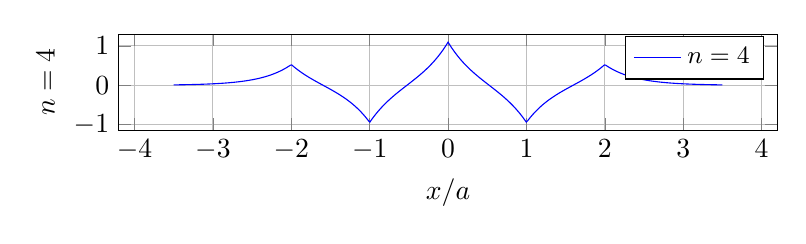
\begin{tikzpicture}
\begin{axis}[width=.82\textwidth,height=2.8cm,xlabel={$x/a$},ylabel={$n=4$},grid=major,legend style={font=\small},]
\addplot+[mark=none] coordinates{(-3.5,0.00986603201) (-3.4825,0.0103342604) (-3.465,0.0108247102) (-3.4475,0.0113384361) (-3.43,0.0118765427) (-3.4125,0.0124401871) (-3.395,0.0130305813) (-3.3775,0.0136489948) (-3.36,0.0142967574) (-3.3425,0.0149752619) (-3.325,0.0156859673) (-3.3075,0.0164304018) (-3.29,0.0172101661) (-3.2725,0.018026937) (-3.255,0.0188824707) (-3.2375,0.0197786069) (-3.22,0.0207172724) (-3.2025,0.0217004857) (-3.185,0.022730361) (-3.1675,0.0238091128) (-3.15,0.0249390606) (-3.1325,0.0261226342) (-3.115,0.0273623786) (-3.0975,0.0286609596) (-3.08,0.0300211694) (-3.0625,0.0314459329) (-3.045,0.0329383137) (-3.0275,0.0345015209) (-3.01,0.0361389158) (-2.9925,0.0378540192) (-2.975,0.039650519) (-2.9575,0.0415322782) (-2.94,0.0435033432) (-2.9225,0.0455679522) (-2.905,0.0477305447) (-2.8875,0.0499957708) (-2.87,0.0523685015) (-2.8525,0.0548538388) (-2.835,0.0574571267) (-2.8175,0.0601839631) (-2.8,0.0630402115) (-2.7825,0.0660320134) (-2.765,0.0691658022) (-2.7475,0.0724483163) (-2.73,0.075886614) (-2.7125,0.0794880886) (-2.695,0.0832604843) (-2.6775,0.0872119126) (-2.66,0.0913508704) (-2.6425,0.0956862574) (-2.625,0.100227396) (-2.6075,0.104984051) (-2.59,0.10996645) (-2.5725,0.115185306) (-2.555,0.120651843) (-2.5375,0.126377814) (-2.52,0.132375532) (-2.5025,0.138657893) (-2.485,0.145238406) (-2.4675,0.152131222) (-2.45,0.159351161) (-2.4325,0.166913748) (-2.415,0.174835246) (-2.3975,0.183132687) (-2.38,0.191823913) (-2.3625,0.200927613) (-2.345,0.210463362) (-2.3275,0.220451664) (-2.31,0.230913998) (-2.2925,0.241872859) (-2.275,0.253351813) (-2.2575,0.265375543) (-2.24,0.277969902) (-2.2225,0.291161972) (-2.205,0.30498012) (-2.1875,0.319454058) (-2.17,0.33461491) (-2.1525,0.350495274) (-2.135,0.367129299) (-2.1175,0.384552752) (-2.1,0.402803098) (-2.0825,0.421919581) (-2.065,0.441943305) (-2.0475,0.462917328) (-2.03,0.48488675) (-2.0125,0.50789881) (-1.995,0.51625248) (-1.9775,0.48633391) (-1.96,0.457461091) (-1.9425,0.429571937) (-1.925,0.40260648) (-1.9075,0.376506737) (-1.89,0.351216586) (-1.8725,0.326681646) (-1.855,0.302849161) (-1.8375,0.279667884) (-1.82,0.257087969) (-1.8025,0.235060863) (-1.785,0.213539202) (-1.7675,0.192476709) (-1.75,0.171828093) (-1.7325,0.151548954) (-1.715,0.131595687) (-1.6975,0.111925386) (-1.68,0.0924957554) (-1.6625,0.0732650158) (-1.645,0.054191816) (-1.6275,0.0352351433) (-1.61,0.0163542358) (-1.5925,-0.0024915057) (-1.575,-0.0213426046) (-1.5575,-0.0402395959) (-1.54,-0.0592231133) (-1.5225,-0.0783339765) (-1.505,-0.0976132791) (-1.4875,-0.117102477) (-1.47,-0.136843477) (-1.4525,-0.156878728) (-1.435,-0.17725131) (-1.4175,-0.198005032) (-1.4,-0.219184518) (-1.3825,-0.24083531) (-1.365,-0.263003964) (-1.3475,-0.285738148) (-1.33,-0.309086747) (-1.3125,-0.333099967) (-1.295,-0.357829443) (-1.2775,-0.383328349) (-1.26,-0.409651516) (-1.2425,-0.436855544) (-1.225,-0.464998932) (-1.2075,-0.494142194) (-1.19,-0.524347996) (-1.1725,-0.555681289) (-1.155,-0.588209448) (-1.1375,-0.622002418) (-1.12,-0.657132862) (-1.1025,-0.693676321) (-1.085,-0.731711374) (-1.0675,-0.771319805) (-1.05,-0.812586783) (-1.0325,-0.855601045) (-1.015,-0.900455082) (-0.9975,-0.933138659) (-0.98,-0.883166971) (-0.9625,-0.835094333) (-0.945,-0.788817375) (-0.9275,-0.744236589) (-0.91,-0.701256115) (-0.8925,-0.659783532) (-0.875,-0.619729664) (-0.8575,-0.581008383) (-0.84,-0.543536429) (-0.8225,-0.507233226) (-0.805,-0.472020713) (-0.7875,-0.437823172) (-0.77,-0.404567071) (-0.7525,-0.3721809) (-0.735,-0.340595018) (-0.7175,-0.309741509) (-0.7,-0.279554028) (-0.6825,-0.249967665) (-0.665,-0.2209188) (-0.6475,-0.192344971) (-0.63,-0.164184736) (-0.6125,-0.136377542) (-0.595,-0.108863598) (-0.5775,-0.0815837402) (-0.56,-0.0544793095) (-0.5425,-0.0274920242) (-0.525,-0.000563854192) (-0.5075,0.0263631034) (-0.49,0.0533467488) (-0.4725,0.0804451042) (-0.455,0.107716439) (-0.4375,0.135219393) (-0.42,0.163013105) (-0.4025,0.19115734) (-0.385,0.219712616) (-0.3675,0.248740333) (-0.35,0.27830291) (-0.3325,0.308463914) (-0.315,0.3392882) (-0.2975,0.370842047) (-0.28,0.403193306) (-0.2625,0.43641154) (-0.245,0.470568179) (-0.2275,0.505736666) (-0.21,0.541992626) (-0.1925,0.579414017) (-0.175,0.618081306) (-0.1575,0.658077639) (-0.14,0.699489017) (-0.1225,0.742404488) (-0.105,0.78691633) (-0.0875,0.833120257) (-0.07,0.88111562) (-0.0525,0.931005621) (-0.035,0.982897537) (-0.0175,1.03690295) (4.4408921e-16,1.09313799) (0.0175,1.03690295) (0.035,0.982897537) (0.0525,0.931005621) (0.07,0.88111562) (0.0875,0.833120257) (0.105,0.78691633) (0.1225,0.742404488) (0.14,0.699489017) (0.1575,0.658077639) (0.175,0.618081306) (0.1925,0.579414017) (0.21,0.541992626) (0.2275,0.505736666) (0.245,0.470568179) (0.2625,0.43641154) (0.28,0.403193306) (0.2975,0.370842047) (0.315,0.3392882) (0.3325,0.308463914) (0.35,0.27830291) (0.3675,0.248740333) (0.385,0.219712616) (0.4025,0.19115734) (0.42,0.163013105) (0.4375,0.135219393) (0.455,0.107716439) (0.4725,0.0804451042) (0.49,0.0533467488) (0.5075,0.0263631034) (0.525,-0.000563854192) (0.5425,-0.0274920242) (0.56,-0.0544793095) (0.5775,-0.0815837402) (0.595,-0.108863598) (0.6125,-0.136377542) (0.63,-0.164184736) (0.6475,-0.192344971) (0.665,-0.2209188) (0.6825,-0.249967665) (0.7,-0.279554028) (0.7175,-0.309741509) (0.735,-0.340595018) (0.7525,-0.3721809) (0.77,-0.404567071) (0.7875,-0.437823172) (0.805,-0.472020713) (0.8225,-0.507233226) (0.84,-0.543536429) (0.8575,-0.581008383) (0.875,-0.619729664) (0.8925,-0.659783532) (0.91,-0.701256115) (0.9275,-0.744236589) (0.945,-0.788817375) (0.9625,-0.835094333) (0.98,-0.883166971) (0.9975,-0.933138659) (1.015,-0.900455082) (1.0325,-0.855601045) (1.05,-0.812586783) (1.0675,-0.771319805) (1.085,-0.731711374) (1.1025,-0.693676321) (1.12,-0.657132862) (1.1375,-0.622002418) (1.155,-0.588209448) (1.1725,-0.555681289) (1.19,-0.524347996) (1.2075,-0.494142194) (1.225,-0.464998932) (1.2425,-0.436855544) (1.26,-0.409651516) (1.2775,-0.383328349) (1.295,-0.357829443) (1.3125,-0.333099967) (1.33,-0.309086747) (1.3475,-0.285738148) (1.365,-0.263003964) (1.3825,-0.24083531) (1.4,-0.219184518) (1.4175,-0.198005032) (1.435,-0.17725131) (1.4525,-0.156878728) (1.47,-0.136843477) (1.4875,-0.117102477) (1.505,-0.0976132791) (1.5225,-0.0783339765) (1.54,-0.0592231133) (1.5575,-0.0402395959) (1.575,-0.0213426046) (1.5925,-0.0024915057) (1.61,0.0163542358) (1.6275,0.0352351433) (1.645,0.054191816) (1.6625,0.0732650158) (1.68,0.0924957554) (1.6975,0.111925386) (1.715,0.131595687) (1.7325,0.151548954) (1.75,0.171828093) (1.7675,0.192476709) (1.785,0.213539202) (1.8025,0.235060863) (1.82,0.257087969) (1.8375,0.279667884) (1.855,0.302849161) (1.8725,0.326681646) (1.89,0.351216586) (1.9075,0.376506737) (1.925,0.40260648) (1.9425,0.429571937) (1.96,0.457461091) (1.9775,0.48633391) (1.995,0.51625248) (2.0125,0.50789881) (2.03,0.48488675) (2.0475,0.462917328) (2.065,0.441943305) (2.0825,0.421919581) (2.1,0.402803098) (2.1175,0.384552752) (2.135,0.367129299) (2.1525,0.350495274) (2.17,0.33461491) (2.1875,0.319454058) (2.205,0.30498012) (2.2225,0.291161972) (2.24,0.277969902) (2.2575,0.265375543) (2.275,0.253351813) (2.2925,0.241872859) (2.31,0.230913998) (2.3275,0.220451664) (2.345,0.210463362) (2.3625,0.200927613) (2.38,0.191823913) (2.3975,0.183132687) (2.415,0.174835246) (2.4325,0.166913748) (2.45,0.159351161) (2.4675,0.152131222) (2.485,0.145238406) (2.5025,0.138657893) (2.52,0.132375532) (2.5375,0.126377814) (2.555,0.120651843) (2.5725,0.115185306) (2.59,0.10996645) (2.6075,0.104984051) (2.625,0.100227396) (2.6425,0.0956862574) (2.66,0.0913508704) (2.6775,0.0872119126) (2.695,0.0832604843) (2.7125,0.0794880886) (2.73,0.075886614) (2.7475,0.0724483163) (2.765,0.0691658022) (2.7825,0.0660320134) (2.8,0.0630402115) (2.8175,0.0601839631) (2.835,0.0574571267) (2.8525,0.0548538388) (2.87,0.0523685015) (2.8875,0.0499957708) (2.905,0.0477305447) (2.9225,0.0455679522) (2.94,0.0435033432) (2.9575,0.0415322782) (2.975,0.039650519) (2.9925,0.0378540192) (3.01,0.0361389158) (3.0275,0.0345015209) (3.045,0.0329383137) (3.0625,0.0314459329) (3.08,0.0300211694) (3.0975,0.0286609596) (3.115,0.0273623786) (3.1325,0.0261226342) (3.15,0.0249390606) (3.1675,0.0238091128) (3.185,0.022730361) (3.2025,0.0217004857) (3.22,0.0207172724) (3.2375,0.0197786069) (3.255,0.0188824707) (3.2725,0.018026937) (3.29,0.0172101661) (3.3075,0.0164304018) (3.325,0.0156859673) (3.3425,0.0149752619) (3.36,0.0142967574) (3.3775,0.0136489948) (3.395,0.0130305813) (3.4125,0.0124401871) (3.43,0.0118765427) (3.4475,0.0113384361) (3.465,0.0108247102) (3.4825,0.0103342604) (3.5,0.00986603201)};
\addlegendentry{$n=4$}
\end{axis}\end{tikzpicture}\end{center}

\originalsection{Rayleigh商与单点势Gaussian例}
非归一试态的正确能量泛函是$F[\phi]=\langle\phi,H\phi\rangle/\langle\phi,\phi\rangle$. 在完整能态基展开即得$F\ge E_0$; 对态变化求一阶驻点给$(H-F)\phi=0$, 所有本征态均为驻点. 激发态通常是鞍点, 若准确正交于较低态, 才给对应激发能上界; 8.05作业2第3题给二阶展开.

对$V=-\alpha\delta(x)$, $\alpha>0$, 取$\phi_\beta=\e^{-\beta^2x^2/2}$, $\beta>0$. 分别计算范数$\sqrt\pi/\beta$, 动能分子$\hbar^2\beta\sqrt\pi/(4m)$, 势能分子$-\alpha$, 得
\[
F(\beta)=\frac{\hbar^2\beta^2}{4m}-\frac{\alpha\beta}{\sqrt\pi},
\quad \beta_*=\frac{2m\alpha}{\hbar^2\sqrt\pi},
\quad F_{\min}=-\frac{m\alpha^2}{\pi\hbar^2}.
\]
二次函数开口向上, 驻点为全局最小. 精确跳跃解$E_0=-m\alpha^2/(2\hbar^2)$, 所以$F_{\min}=(2/\pi)E_0$更接近0而高于$E_0$; 负数大小不能看绝对值反转. 普通一维任意吸引势的Gaussian证明见8.05作业2第4题: 宽态动能为$\alpha$阶, 井内负贡献为$\sqrt\alpha$阶, 从而给负Rayleigh商及束缚态存在.
